\documentclass[11pt]{article}
\usepackage[margin=2.2cm]{geometry}
\usepackage[T1]{fontenc}
\usepackage{amsmath,amssymb,booktabs,graphicx,xcolor,enumitem,tikz,caption,longtable,array}
\usepackage[section]{placeins}
\usepackage{hyperref}
\usepackage{xurl}
\usepackage{fvextra}
\fvset{breaklines=true,fontsize=\footnotesize}
\usetikzlibrary{positioning,arrows.meta}
\setlist{itemsep=2pt,topsep=3pt}
\hypersetup{colorlinks=true,linkcolor=blue!50!black,urlcolor=blue!50!black}
\captionsetup{font=small,labelfont=bf}
\definecolor{trace}{HTML}{2A78D6}
\definecolor{image}{HTML}{C9551F}
\definecolor{model}{HTML}{13865D}
\definecolor{ink2}{HTML}{4A5462}
\tikzset{
  box/.style={draw=#1,fill=#1!8,rounded corners=3pt,align=center,font=\footnotesize,minimum height=1cm,text width=2.0cm,line width=0.7pt},
  box/.default=ink2,
  arr/.style={-{Stealth[length=2.2mm]},line width=0.8pt,color=ink2},
}
\setlength{\emergencystretch}{3em}
\newcommand{\hyp}[1]{\textit{#1}}

\title{The v2 data set: what it is, what it will train, and what we expect to learn}
\author{ccd\_opt\_ml, level 1}
\date{Plan of 2026-11-04, for the first v2 night}

\begin{document}
\maketitle

\section*{Summary}
The v2 night is 76 packets (about 21 hours) on board 101 of PA03, designed from what the first night (43 packets,
2026-11-02/03) taught us. Every packet takes reference traces at nominal settings, a reference level-1 strip, a change of
\emph{all} twelve knob groups at once, settling traces, new traces, a new level-1 strip, and a 32-row image, with
flushes around every step and automatic retakes of damaged traces. The data will be used for four things:
\begin{enumerate}
\item \textbf{Absolute prediction} (task A): predict the image's $\sigma_e$, $\lambda$ and gain from the traces, from the
  level-1 strip, and from both, on the same packets; choose models on session D, test once on session E.
\item \textbf{Change prediction} (task B): given two traces of the same amplifier, predict how $\sigma_e$, $\lambda$ and
  the gain change between them, in size and direction.
\item \textbf{Transfer} (task C): predictions for an amplifier, and if possible a CCD, the models never saw.
\item \textbf{Diagnostics} (task D): label noise at every setting, learning curves, what each model relies on.
\end{enumerate}
The main expectations: $\sigma_e$ should be predicted from the traces to about the 5\,\% level and keep transferring;
the strip should measure the gain and the clock-induced part of $\lambda$ directly; the size (not only the direction) of
changes should become predictable once the drift is tracked and there are five times more examples.

\tableofcontents

% =====================================================================================================
\section{The questions v2 has to answer}

The first night established a pipeline and three results (first-data report, level-1 summary): (i) the trace predicts
$\sigma_e$ through its measured white noise, also on amplifiers it never saw; (ii) the gain and the \emph{level} of
$\lambda$ were predicted mostly by recognising the amplifier, which cannot carry over to a new one, and the gain is not
in a trace at all (no known charge); (iii) the \emph{direction} of a change of $\sigma_e$ and $\lambda$ between two traces
taken minutes apart is right about 9 times in 10, but its size is not reliably predicted. v2 is built to answer:

\begin{description}
\item[Q1. Which cheap measurement predicts the image?] Traces only, a level-1 strip only, or both, compared on the same
  packets, rows and folds.
\item[Q2. Can the change between any two traces be predicted,] in size and not only in direction? With drift tracked,
  clean change labels from the strips, and about five times more examples.
\item[Q3. Does it carry over?] To an amplifier the model never saw, and to a second CCD if its settings are varied too.
\item[Q4. Is more data still helping?] The learning curve was still falling at 32 packets.
\item[Q5. How good are the labels?] Repeat scatter at every setting (replicates), not only at nominal.
\end{description}

% =====================================================================================================
\section{What changes from the first night, and why}

\begin{longtable}{p{3.2cm}p{5.3cm}p{6.7cm}}
\toprule
change & v2 & the first-night lesson behind it\\\midrule
\endhead
joint design & all 12 knob groups move at once, to points of a scrambled Sobol sequence (timing on a log scale) &
  one-knob-at-a-time packets made cross-validation test extrapolation; the model chosen on them failed on session C,
  which changed knobs jointly\\
more distinct settings & 38--48 distinct levels per knob in session D & each knob had about one value in v1; boosted
  trees could not split on knobs changed in 1--2 packets\\
nominal every 7 packets & 10 in session D, 3 in E & $\lambda$ fell about 20\,\% over the night at fixed settings; drift
  must be tracked and modelled\\
replicates & 3 design points repeated later in D & label noise was known only at nominal\\
session E & a separate Sobol sequence, scored once & the prospective test that exposed the extrapolation problem\\
flushes & before and after the reference traces, before and after the image & L1\_18 waited 38 minutes without a flush
  and its $\lambda$ was four times too high\\
settling traces & 2 traces after the change, not used & the first traces after a change carry the transition\\
3 + 5 trace sets & instead of 5 + 10 & time goes to strips and more packets; damaged traces are retaken instead\\
safeguards & damaged traces retaken; more than 5 restarts the packet & three session-C packets lost every trace at their
  settings\\
level-1 strips & a reference and a new strip in every packet & the trace has no known charge (no gain) and does not see
  what the image's pixels go through after the prescan and clear\\
32-row image & instead of 16 & twice the pixels; the dark-current part of $\lambda$ about 3$\times$ better\\
pauses & 2 s after every trace and image & to let the boards settle between acquisitions\\\bottomrule
\end{longtable}

% =====================================================================================================
\section{The v2 packet}

\subsection{Sequence}
\begin{center}
\resizebox{\textwidth}{!}{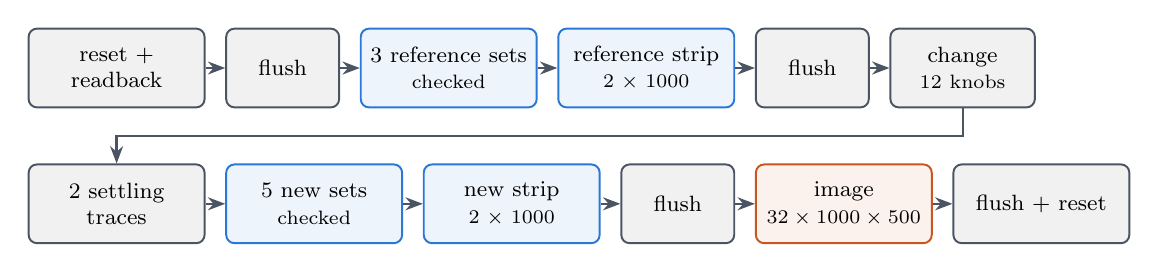
\begin{tikzpicture}[node distance=0.25cm]
\node[box] (a) {reset + readback};
\node[box,right=of a,text width=1.2cm] (b) {flush};
\node[box=trace,right=of b] (c) {3 reference sets\\\scriptsize checked};
\node[box=trace,right=of c] (d) {reference strip\\\scriptsize $2\times1000$};
\node[box,right=of d,text width=1.2cm] (e) {flush};
\node[box,right=of e,text width=1.6cm] (f) {change\\\scriptsize 12 knobs};
\node[box,below=0.7cm of a] (g) {2 settling traces};
\node[box=trace,right=of g] (h) {5 new sets\\\scriptsize checked};
\node[box=trace,right=of h] (i) {new strip\\\scriptsize $2\times1000$};
\node[box,right=of i,text width=1.2cm] (j) {flush};
\node[box=image,right=of j] (k) {image\\\scriptsize $32\times1000\times500$};
\node[box,right=of k] (l) {flush + reset};
\foreach \x/\y in {a/b,b/c,c/d,d/e,e/f,g/h,h/i,i/j,j/k,k/l} \draw[arr] (\x)--(\y);
\draw[arr] (f.south) -- ++(0,-0.35) -| (g.north);
\end{tikzpicture}}
\end{center}
A packet takes 10--23 minutes depending on the timing settings (a longer integration window makes every skip slower);
nominal packets about 16 minutes. The plan (lvl1/packet\_plan\_v2/, made by lvl1/make\_packet\_plan\_v2.py) has
session D, 61 packets (10 nominal, 17.1 h) for training and model choice, and session E, 15 packets (3 nominal, 4.3 h)
for the prospective test. daq\_scripts/run\_plan.sh takes them in order, skips finished packets, and stops on an error or
a STOP file.

\subsection{The knob box}
\begin{center}\small
\begin{tabular}{llp{8.5cm}}\toprule
knob & range & why it matters\\\midrule
delayInt & 300--3000 cycles (log) & the CDS integration window: white noise falls with a longer window, slow noise grows; the strongest noise knob, and it moves the gain\\
delay\_H & 900--3600 cycles (log) & horizontal clock hold: charge transfer, horizontal clock-induced charge\\
delayRGH & 400--1600 cycles (log) & reset-gate hold before the pedestal window: reset settling\\
VDD & $\pm$1 V & output drain: amplifier operating point (noise, gain)\\
VR & $\pm$0.5 V & reset drain: reset level and its noise\\
VSUB & $\pm$5 V & substrate: depletion, dark current\\
RG\_H, RG\_L & $\pm$0.5 V & reset-gate rails\\
SW\_L & $-0.5$--0 V & summing-well low rail\\
H\_low & $\pm$0.5 V & horizontal clock low rails: clock-induced charge\\
V\_low & 0--0.5 V & vertical clock low rails: clock-induced charge, surface dark current\\
TG & $\pm$0.25 V & transfer gate\\\bottomrule
\end{tabular}
\end{center}

\subsection{What each packet gives}
\begin{center}\small
\begin{tabular}{p{4.2cm}p{4.0cm}p{6.8cm}}\toprule
product & per amplifier & used for\\\midrule
3 reference trace sets & features + curves at nominal & the amplifier's state just before the change; the ``A'' side of a within-packet change\\
5 new trace sets & features + curves at the new setting & task A inputs; the ``B'' side of a change\\
reference strip & strip features at nominal & the strip's own $\sigma_e$, gain, CIC at nominal\\
new strip & strip features at the new setting & task A strip inputs; with the reference strip, a \emph{measured} within-packet change of gain and CIC\\
image & $\sigma_e$, $\lambda$, gain (WADERs); $\lambda$ per row & the labels\\
record, readback & settings, times, status & bookkeeping, drift time axis, quality\\\bottomrule
\end{tabular}
\end{center}

\section{Before the night}
\begin{enumerate}
\item \textbf{DAQ strip test}: take $1\times500$, $1\times1000$ and $2\times1000$ level-1 strips by hand and check that all
  rows arrive complete (src/check\_trace\_files.py \texttt{--l1}); manual\_packet.sh uses $2\times1000$ by default.
\item \textbf{Code on the DAQ machine}: pull main; copy configs/image\_params\_32rows.toml to
  image\_params/tc1/img32.toml.
\item \textbf{Settings on every working board}: the plan changes board 101 only. To test transfer to a second CCD
  (task C), the changes must also be applied to a second working module; otherwise task C can only use new amplifiers
  on board 101.
\item \textbf{Voltage windows}: configs/limits.toml is still marked \texttt{reviewed = false}.
\item \textbf{Temperature}: log the CCD temperature per packet if a readout exists; it drives dark current and drift.
\item \textbf{Bad channels}: decide on board 101 ch2 (EXT3) before training (its per-row fit $\chi^2$ is 22, others
  3--4); the current recommendation is to leave it out of training and report it separately.
\end{enumerate}

% =====================================================================================================
\section{From raw files to training inputs}

Processing is unchanged from the first night, plus the strips: make\_manual\_manifest.py (lists traces, strips, image;
skips restarted attempts), process\_packet.py (decodes and checks traces, features, strip features, WADERs labels with
the drift correction off, $\lambda$ per row), real\_inputs.py (one file per model family). It writes three input folders on
exactly the same rows: \texttt{model\_inputs} (traces), \texttt{model\_inputs\_l1} (strip features in place of trace
features) and \texttt{model\_inputs\_both}. A row needs a usable trace \emph{and} a usable strip at its own settings.

\paragraph{Default training choices} (from the 2026-11-04 tests): traces only, never the settings as an input
(\texttt{--no-settings}; neutral or better for the physics model and the networks); without the amplifier-fingerprint
features (\texttt{--exclude-features}, list recomputed on v2); without unreliable amplifiers
(\texttt{--exclude-amps}). The labelled references (settings + amplifier name) are still run, as references.

% =====================================================================================================
\section{Task A: predicting the image from a trace, a strip, or both}

\subsection{Targets and error}
Per amplifier and packet, $y=(\log\sigma_e,\log\lambda,\log g)$ from the image; the error of a model is
\[\mathrm{error}=100\sqrt{\tfrac1n\textstyle\sum(\hat y-y)^2}\ \%,\]
a typical relative error.

\subsection{Models}
All existing families (first-data report, appendix A): the average and the labelled references; ridge, boosted trees,
GP, gp\_dim and network ensembles on features; cnn, the pre-trained encoder and the deep-kernel GP on curves; the
physics-structured family. The default is \texttt{physics\_white}:
\begin{equation}
\log\hat\sigma_e=\tfrac12\log\frac{w^2}{N}-\log\hat g(x)+\hat r(x),\qquad \log\hat\lambda=\hat f_\lambda(x),\qquad \log\hat g=\log\hat g(x),
\end{equation}
with $w$ the trace's white noise per skip, $N$ the image's skips, and GPs for $\hat g$, the correction $\hat r$ and
$\lambda$ (SAAS). For the strip source the same structure applies with the strip's own white noise, and the strip's
measured gain and $\lambda$ become inputs of $\hat g$ and $\hat f_\lambda$.

\subsection{Protocol}
\begin{enumerate}
\item Setting-grouped cross-validation on session D (packets at identical settings, i.e.\ replicates and nominal repeats,
  share a fold), for every model, every feature tier and every source.
\item Choose per target the model and feature set with the lowest CV error; write the choice to git (frozen).
\item Score session E once; paired packet bootstrap against the no-trace references and between the three sources.
\item Explain the chosen models (lvl1/explain\_models.py: fitted parameters, input shuffles).
\end{enumerate}
Because D and E are both joint designs, cross-validation on D now measures the same kind of generalisation as the test
on E, which was not true in v1.

\subsection{What we expect}
\begin{itemize}
\item \textbf{$\sigma_e$ from traces}: the learning curve on v1 fell from 9.7 to 5.9\,\% between 8 and 32 packets;
  with 61 jointly designed packets we expect about 4--6\,\% on session E, approaching twice the label scatter (about
  4\,\%). The timing packets carried most of the v1 error; the strip, read exactly like the image, should remove most of
  it, so we expect \emph{both} $<$ \emph{traces}.
\item \textbf{Gain}: from the strip's peak spacing directly, at about 1\,\%; traces alone will stay at the level of
  ``the average'' on new amplifiers, by physics.
\item \textbf{$\lambda$}: the strip measures the clock-induced and serial-register part (about 75\,\% of $\lambda$ on
  board 101); the image's dark current (rows waiting during readout) still has to be predicted, and the night's drift
  is now tracked by the nominal packets. We expect $\lambda$ to improve most from strips.
\end{itemize}

\begin{figure}[h]
\centering
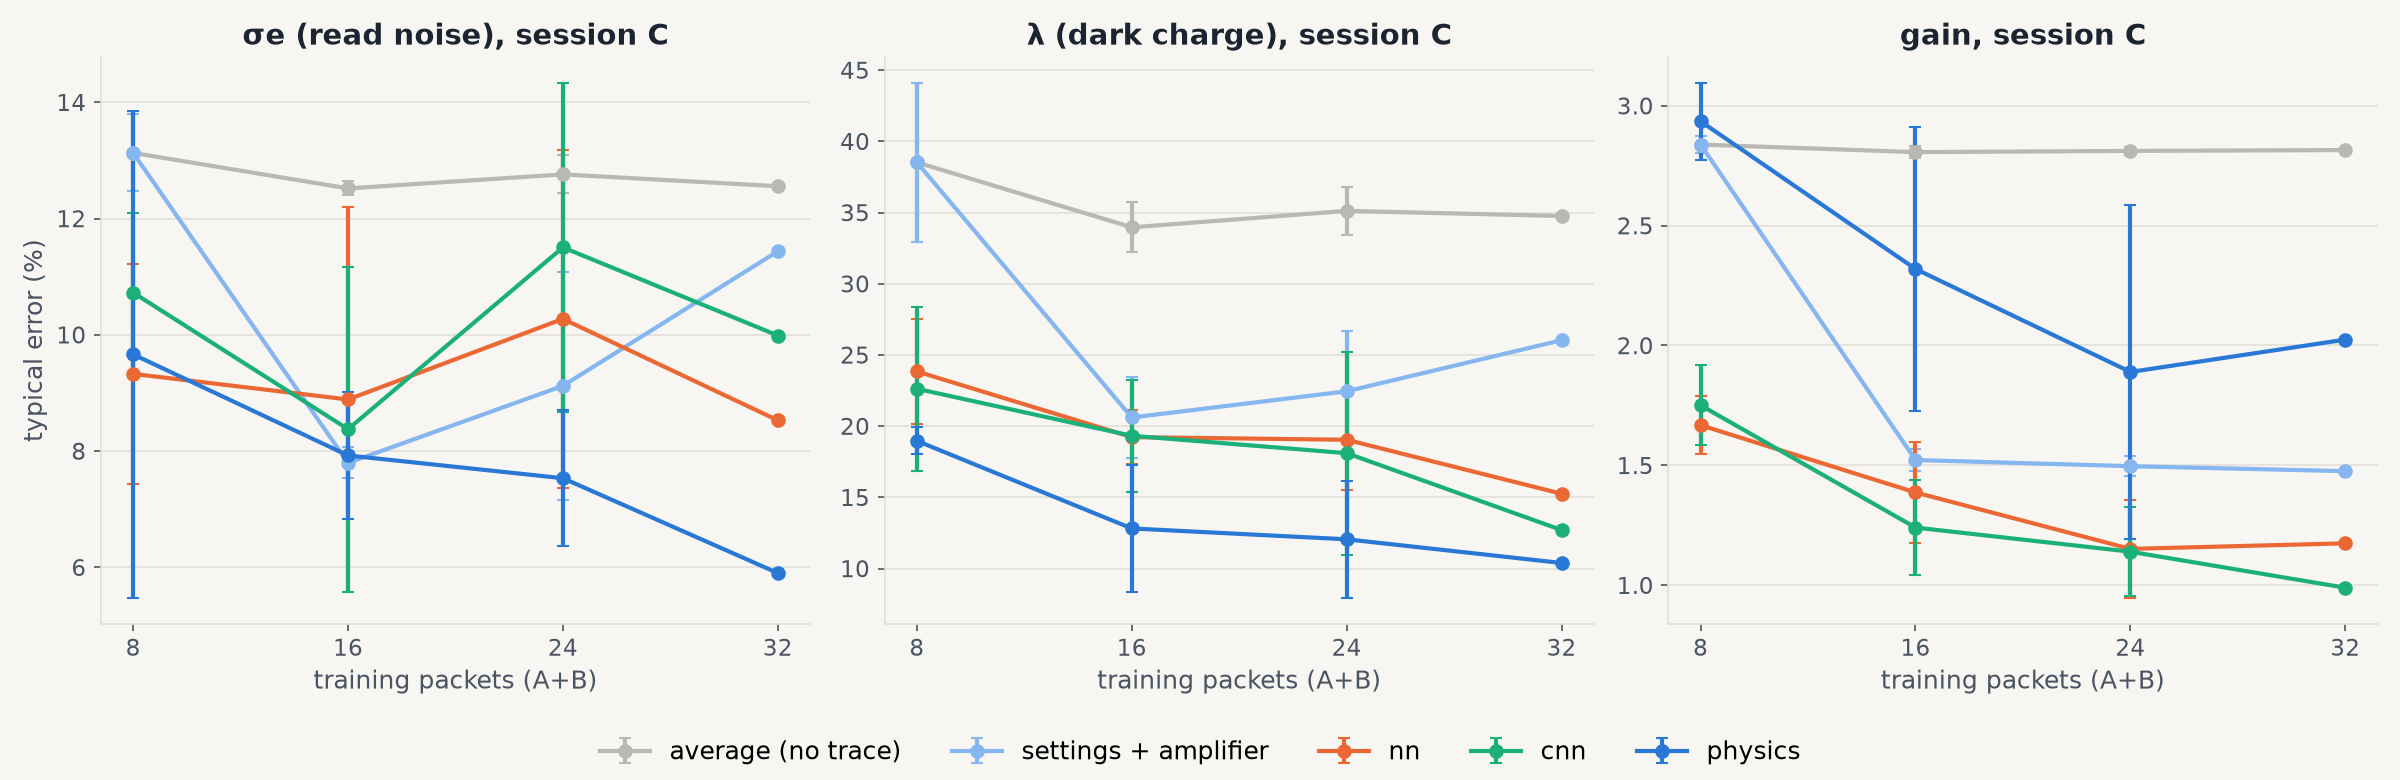
\includegraphics[width=\textwidth]{figures/fig_learning_curve.png}
\caption{Learning curve on the first night (session C error against the number of training packets, without ch2 and
the fingerprint features): still falling at 32 packets.}
\end{figure}

% =====================================================================================================
\section{Task B: predicting the change between two traces}

\subsection{The question}
Given two traces of the same amplifier, $A$ and $B$ (any two settings, not necessarily nominal), predict
\begin{equation}
\Delta=\log y(B)-\log y(A)
\end{equation}
for $y=\sigma_e,\lambda,g$: its size, and at least its direction (up or down). This is what an optimiser needs (``is
setting B better than A?''), it does not need any amplifier's absolute level, and comparing two traces of the same
amplifier cancels its fingerprint.

\subsection{Where the change labels come from}
\begin{description}
\item[Within a packet, from the strips.] The reference strip (at nominal) and the new strip (at the new setting) are
  minutes apart and both have electron peaks, so $\Delta g$, $\Delta$CIC and the strip's $\Delta\sigma_e$ are
  \emph{measured} directly, without drift and without any nominal image. This is new in v2 and is the cleanest change
  label we will have.
\item[Within a packet, from the images.] $\Delta$ between the packet's image and the same amplifier's nominal level
  interpolated in time between the neighbouring nominal packets (now every 7 packets, so the interpolation spans about
  2 hours instead of 4--6).
\item[Between packets.] Any two packets of one amplifier, both with an image: $\Delta=\log y_j-\log y_i$ with both labels
  measured. Pairs are limited in time (within an hour, or neighbouring packets), because the drift over hours swamps the
  setting's effect (first-night test: direction right 88\,\% within a packet and within an hour for $\lambda$, 66--75\,\%
  for any two packets).
\end{description}

\subsection{Models}
\begin{itemize}
\item \textbf{Difference inputs}: the change of each trace feature (log ratio for positive features) between $A$ and
  $B$, with boosted trees or a GP.
\item \textbf{Shared encoder (``Siamese'')}: one network $g$ scores a single trace, and $\hat\Delta=g(B)-g(A)$, so
  swapping the traces flips the sign by construction. Inputs to $g$: the trace features, or the curves through the CNN
  encoder pre-trained on all unlabelled traces. Losses:
\begin{align}
\text{size:}\quad & \mathcal L=\mathrm{Huber}\big(\hat\Delta-\Delta\big),\\
\text{direction:}\quad & \mathcal L=w\,\log\!\big(1+e^{-\kappa\,\mathrm{sign}(\Delta)\,\hat\Delta}\big),\qquad w=1-e^{-\Delta^2/2s^2},
\end{align}
  with $s$ the label noise of a change, so a change of the size of the noise counts little; ``both'' adds them.
\item \textbf{Difference curves}: the 16 curves of $B$ minus those of $A$ (standardized per point), either reduced to their
  main patterns (PCA) or reduced to a few hand-picked bands chosen on the training rows, where the change of the target
  correlates most with the difference curve (Figure~\ref{fig:dcorr}).
\item \textbf{Physics difference} for $\sigma_e$: $\hat\Delta\log\sigma_e=\Delta\log w-\widehat{\Delta\log g}$, plus a
  learned correction.
\item \textbf{References}: ``no change'' ($\hat\Delta=0$) and the same learners on the settings change.
\end{itemize}

\begin{figure}[h]
\centering
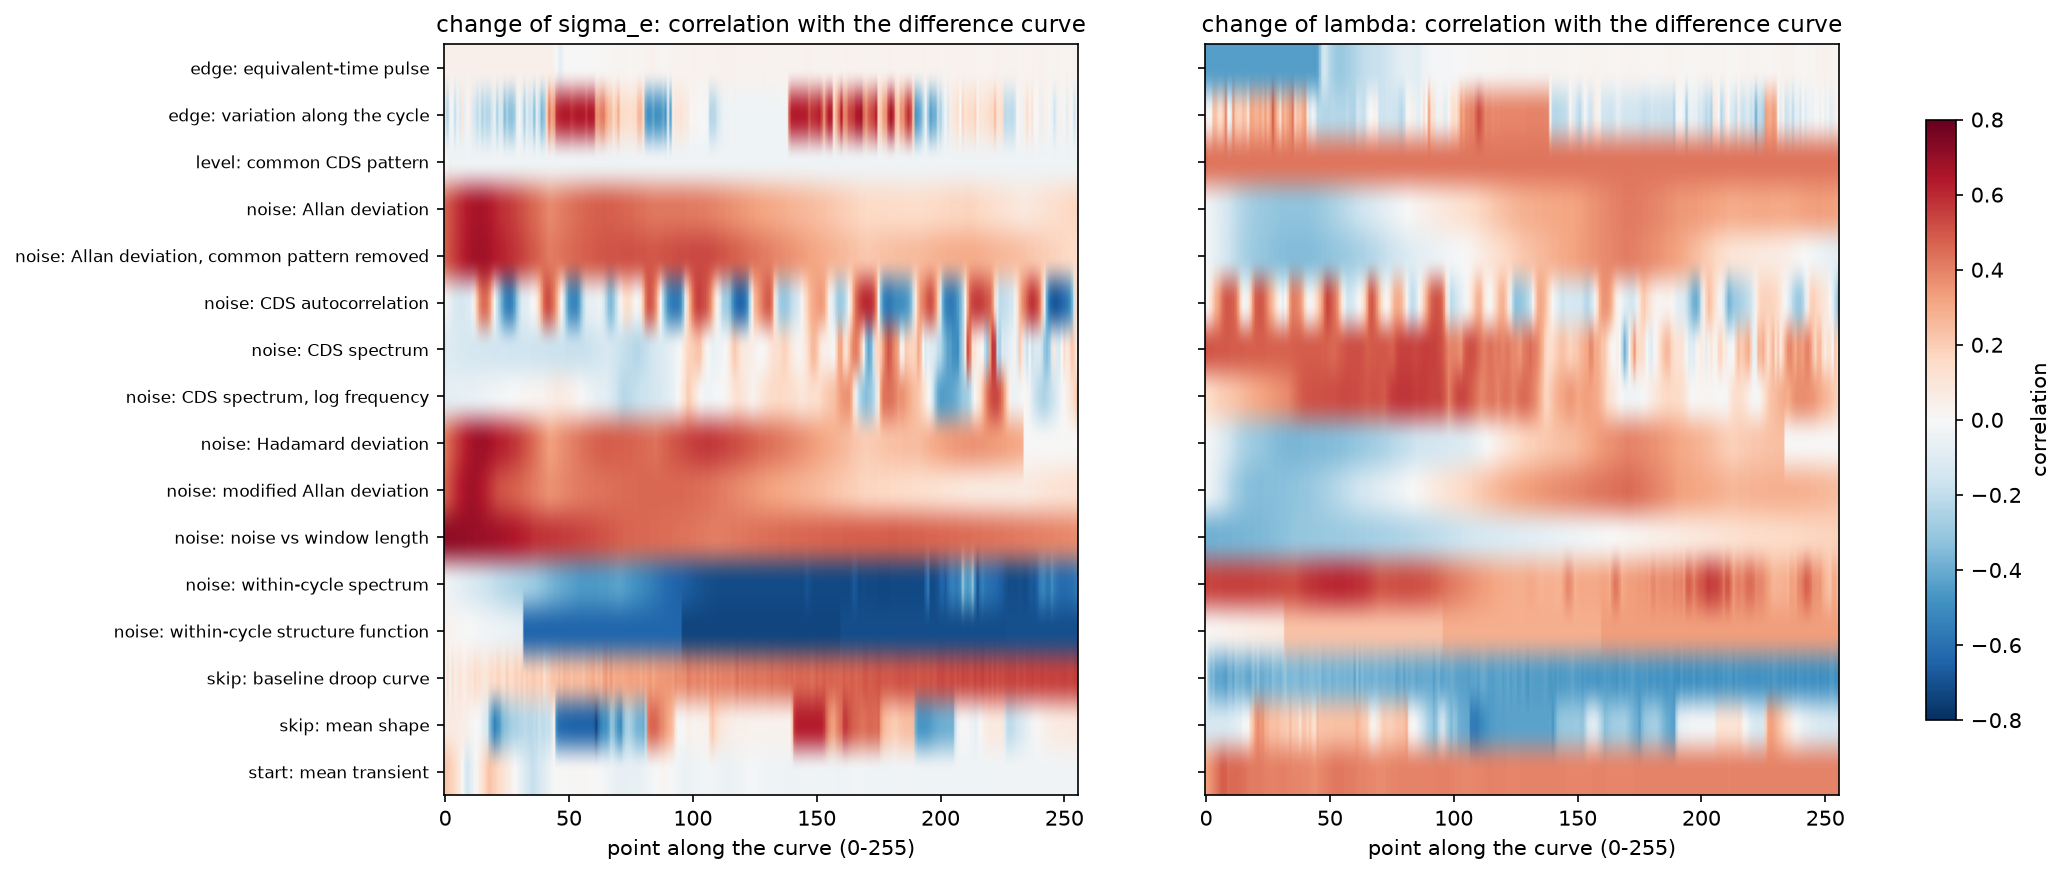
\includegraphics[width=0.9\textwidth]{figures/difference_curve_correlation.png}
\caption{First night: where along each difference curve (new minus reference) the change of $\sigma_e$ (left) and
$\lambda$ (right) is correlated. $\Delta\sigma_e$ follows the mean skip shape, the within-cycle noise and noise against
window length; $\Delta\lambda$ the within-cycle and CDS spectra.}
\label{fig:dcorr}
\end{figure}

\subsection{Scores}
For every model and target: the RMS error of $\Delta$, its median absolute error (less sensitive to a few large
changes), the fraction of \emph{clear} changes (larger than about twice the label noise of a change) whose direction is
right, and the Spearman correlation between predicted and true changes. Always on amplifiers not in training (task C).

\subsection{What we expect}
On the first night most changes were smaller than the label noise of a change (median true change $\sigma_e$ 3.9\,\%,
$\lambda$ 8.5\,\%, gain 0.4\,\%, against label noise 1.9, 11.9 and 0.8\,\%), and there were 84 examples. v2 changes
twelve knobs at once over a wider box, so changes are larger; the strips give drift-free change labels; and there are
about five times more examples. We therefore expect:
\begin{itemize}
\item the \textbf{direction} of $\sigma_e$ and $\lambda$ changes to stay at 85--95\,\% and the gain's to become
  measurable from the strips;
\item the \textbf{size} of $\sigma_e$ changes to be predicted clearly better than ``no change'', and the size of
  $\lambda$ changes to become predictable at least for the large ones;
\item the shared-encoder models, which overfitted 84 examples, to become competitive.
\end{itemize}

\subsection{Check on the first night: neighbouring packets}
Before relying on cross-packet pairs, the first-night data were tested with pairs of \emph{neighbouring} packets of the
same amplifier: packet $n$ against $n\pm1$, and against $n\pm2$ (lvl1/change\_pairs.py \texttt{--max-step},
\texttt{--block-folds}), next to the within-packet change (new trace against the packet's nominal reference). Both
labels of a neighbouring pair are measured. Board 101 without ch2, sessions A+B; a new amplifier (trained on the other
amplifiers); folds are contiguous blocks of packets in time so neighbours stay together.

\begin{center}\small
\begin{tabular}{lcccccc}\toprule
 & \multicolumn{3}{c}{direction right (clear changes)} & \multicolumn{3}{c}{typical error of the size (\%)}\\
pairs, model & $\sigma_e$ & $\lambda$ & gain & $\sigma_e$ & $\lambda$ & gain\\\midrule
within a packet, trace change (trees) & 94\,\% & 88\,\% & 64--82\,\% & 12.6 & 38.9 & 0.9\\
within a packet, no change & -- & -- & -- & 18.5 & 36.8 & 0.9\\\midrule
$n\pm1$, trace change (GP) & 75\,\% & 84\,\% & 81\,\% & 10.3 & 51.8 & 1.3\\
$n\pm1$, trace change (trees) & 66\,\% & \textbf{91\,\%} & 81\,\% & 11.6 & 47.6 & 1.2\\
$n\pm1$, settings change (GP) & 53\,\% & 82\,\% & 81\,\% & 12.2 & 52.2 & 1.0\\
$n\pm1$, no change & -- & -- & -- & 11.6 & 50.6 & 1.3\\\midrule
$n\pm2$, trace change (trees) & 71\,\% & 86\,\% & 76\,\% & 12.6 & 47.2 & 1.2\\
$n\pm2$, settings change (trees) & 78\,\% & 78\,\% & 59\,\% & 12.4 & 46.7 & 1.3\\
$n\pm2$, no change & -- & -- & -- & 14.8 & 52.3 & 1.2\\\bottomrule
\end{tabular}
\end{center}
Number of clear changes: $n\pm1$: 32 ($\sigma_e$), 44 ($\lambda$), 21 (gain); $n\pm2$: 68, 85, 41.

\paragraph{What it shows.} Between neighbouring packets the trace change gets the direction of $\lambda$ right 91\,\% of the
time (settings alone: 50--82\,\%) and the gain's 81\,\%; $\sigma_e$'s direction is clearly better within a packet (94\,\%)
than between packets (66--75\,\%), because the reference and new traces of a packet are minutes apart. The \emph{size} of
the change is still no better than ``no change'' for $\lambda$ (the RMS is dominated by L1\_18, the stalled packet) and
only slightly better for $\sigma_e$ (GP 10.3 against 11.6\,\%). So for v2: within-packet pairs are the core training set
for $\sigma_e$; neighbouring pairs add useful examples for $\lambda$ and the gain; pairs far apart in time should not be
used.


% =====================================================================================================
\section{Task C: does it carry over?}

\begin{itemize}
\item \textbf{New amplifier}: leave one amplifier out, crossed with the packet folds (no test packet in training).
  On the first night only the $\sigma_e$ physics model beat the average on a new amplifier (14\,\% against 19\,\%);
  without ch2 and the fingerprints, $\lambda$ beat it too (40\,\% against 52\,\%).
\item \textbf{New CCD}: only if a second working module's settings are changed in v2 (section 4). Then: train on board 101,
  test on the other board, for tasks A and B.
\item \textbf{Expected}: $\sigma_e$ (from the trace's own noise) and the changes (task B, which cancel each amplifier's
  level) should carry over; absolute gain and $\lambda$ levels from traces alone should not, by physics, but the strip
  supplies them.
\end{itemize}

\begin{figure}[h]
\centering
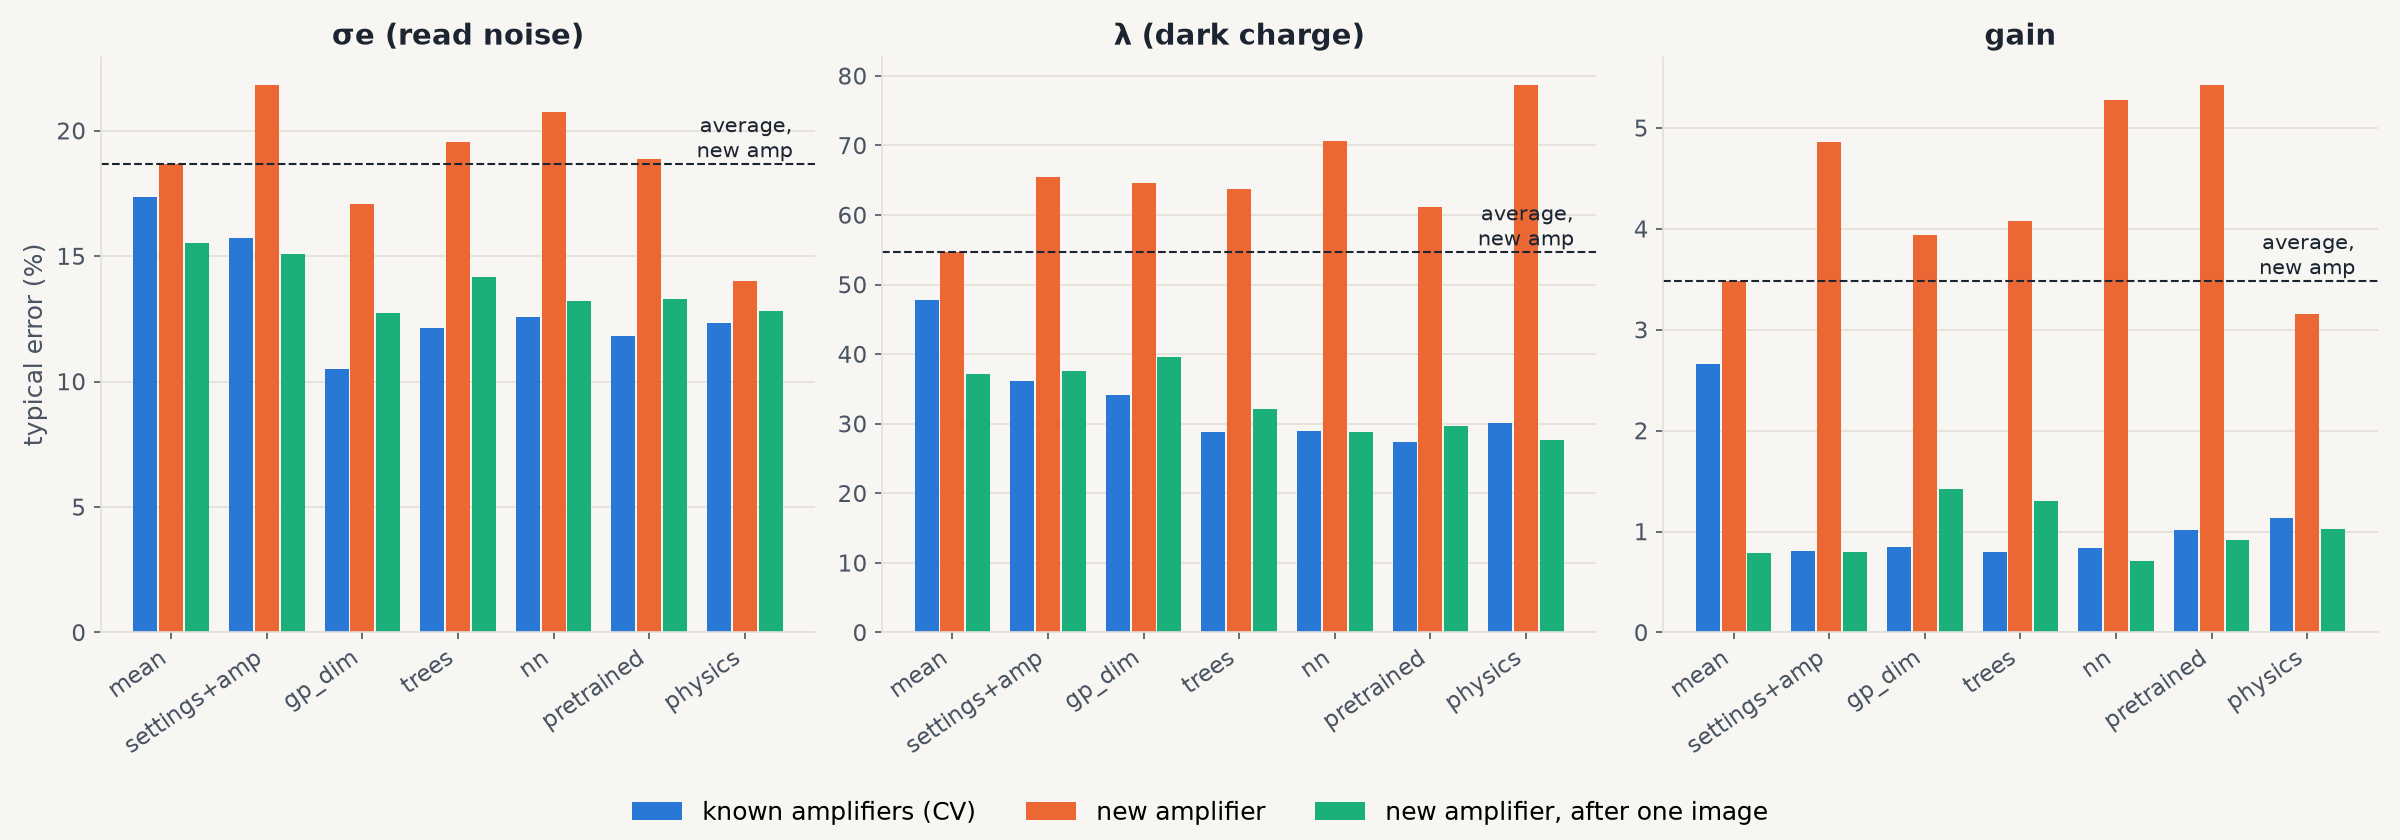
\includegraphics[width=\textwidth]{figures/fig_loao.png}
\caption{First night, leave one amplifier out: error on known amplifiers, on a new amplifier, and after one
calibration image.}
\end{figure}

% =====================================================================================================
\section{Task D: diagnostics}
\begin{itemize}
\item \textbf{Label noise at every setting}: the 3 replicates and 13 nominal packets give the repeat scatter of
  $\sigma_e$, $\lambda$ and gain away from nominal; models are judged against it.
\item \textbf{Drift}: $\lambda$ and the gain of the nominal packets against time (and temperature, if logged).
\item \textbf{Learning curve}: random subsets of 8--61 packets of session D, scored on E; tells whether a third night is
  worth taking.
\item \textbf{What the models rely on}: input shuffles across all rows and within each amplifier; fingerprint list
  recomputed on v2.
\item \textbf{Strip vs image}: the strip's $\sigma_e$, gain and $\lambda$ against the image's, per amplifier.
\end{itemize}

% =====================================================================================================
\section{Outcomes and decisions}
\begin{center}\small
\begin{tabular}{p{6.6cm}p{8.4cm}}\toprule
if v2 shows & then\\\midrule
both $\approx$ strip $\ll$ traces for gain and $\lambda$; traces $\approx$ both for $\sigma_e$ & scan settings with
  traces for $\sigma_e$; take a strip where gain or $\lambda$ matter\\
the change of $\sigma_e$ and $\lambda$ is predicted in size from two traces & level 2 can compare settings from traces
  alone (``is B better than A?'')\\
only the direction is predicted & level 2 uses ranking (preference) optimisation, not regression\\
the learning curve is still falling at 61 packets & take a third night (or a longer one)\\
$\sigma_e$ and changes carry over to a second CCD & build level 2 on the trace models\\
they do not & per-CCD training, or a short calibration session per CCD\\\bottomrule
\end{tabular}
\end{center}
Level 1 passes if, on session E, the trace (alone or with the strip) predicts $\sigma_e$ and $\lambda$ significantly better
than the no-trace references, within about twice the label scatter, and the direction of clear changes is right at least
85\,\% of the time on amplifiers not in training.

\section{Risks}
\begin{itemize}
\item \textbf{Strips do not arrive complete} at $2\times1000$: fall back to $1\times1000$ (the DAQ test decides).
\item \textbf{Damaged traces}: the retakes and restarts cost time; about 1 packet in 10 is expected to restart.
\item \textbf{Night too short}: the plan is 21.4 h; run\_plan.sh can be stopped and resumed; session E must not be cut.
\item \textbf{Drift larger than expected}: the nominal packets every 7 still allow interpolation; flag packets taken after
  long stalls.
\item \textbf{Voltage windows}: the box uses provisional windows; a reviewed limits file must exist before the night.
\end{itemize}

\section{Commands}
\begin{Verbatim}
# on the DAQ machine
DRY_RUN=1 bash daq_scripts/run_plan.sh              # check every packet first
bash daq_scripts/run_plan.sh                        # take the night (STOP file to pause)
# processing (analysis machine)
python src/make_manual_manifest.py ...; python src/process_packet.py ...; python -m ml.real_inputs processed_v2
# task A, three sources, no settings, no fingerprints, cross-validation on D, test once on E
python lvl1/train_lvl1.py --inputs processed_v2/model_inputs[_l1|_both] --no-settings \
    --exclude-features lvl1/feature_study/real_AB/amp_fingerprint_eta90.txt --holdout-session E --loao
# task B
python lvl1/change_models.py; python lvl1/change_handpicked.py; python lvl1/change_pairs.py --max-step 1
# task D
python lvl1/learning_curve.py ...; python lvl1/explain_models.py ...; python lvl1/amp_fingerprint.py
\end{Verbatim}
(The scripts read the v1 paths today; pointing them at the v2 folders is part of the processing step.)

\end{document}
